\documentclass[sigconf]{acmart}

\title{Enhanced Predictive Maintenance for Hydraulic Systems Using Machine Learning}

\author{Rock Deng}
\affiliation{%
  \institution{University of Colorado Boulder}}
\email{dengyongpeng110@outlook.com}

\begin{document}

\begin{abstract}
Hydraulic systems are critical components in industrial applications, and unexpected failures can lead to costly downtime. This project leverages machine learning techniques for predictive maintenance using the Condition Monitoring of Hydraulic Systems dataset. The objective is to classify failure risks and suggest preventive measures by implementing various machine learning techniques, including decision trees, XGBoost, and time-series models. This study introduces a systematic data preprocessing approach, feature engineering, and model comparison to improve predictive accuracy while ensuring computational efficiency. Moreover, our work builds on previous research by incorporating principal component analysis (PCA) for feature reduction, optimizing model efficiency for real-time monitoring, and providing a comparative analysis of feature importance across models. Finally, we discuss challenges encountered and propose future directions for further enhancing predictive maintenance solutions in industrial settings.
\end{abstract}

\maketitle

\section{Introduction}
Hydraulic systems play a vital role in industrial operations, but their maintenance often relies on reactive or scheduled maintenance, leading to inefficiencies. Predictive maintenance, powered by machine learning, offers an intelligent approach to anticipating failures before they occur. While previous research has focused on various classification models, there remains a gap in optimizing real-time monitoring capabilities. This study aims to implement and evaluate machine learning techniques to develop a predictive maintenance model using the Condition Monitoring of Hydraulic Systems dataset, with a specific focus on optimizing computational efficiency for real-world deployment.


\section{Dataset Description and Exploration} 
The "Condition Monitoring of Hydraulic Systems" dataset provides comprehensive sensor data from a hydraulic test rig, facilitating the analysis and assessment of various component conditions. This dataset is particularly valuable for tasks such as fault detection, predictive maintenance, and machine learning model development.


\subsection{Dataset Overview} 
\begin{itemize} 
    \item \textbf{Source}: The dataset is available through the UCI Machine Learning Repository.
    \item \textbf{Structure}: It comprises multivariate time-series data with 2,205 instances (cycles) and 43,680 features. Each cycle corresponds to a 60-second load sequence, during which various sensor measurements are recorded.
\end{itemize}

\subsection{Key Components Monitored} 
\begin{itemize} 
    \item \textbf{Cooler}: Monitored for efficiency, with conditions ranging from full efficiency (100%) to near-total failure (3%).
    \item \textbf{Valve}: Assessed based on switching behavior, with conditions from optimal (100%) to severe lag (73%).
    \item \textbf{Pump}: Evaluated for internal leakage, categorized as no leakage (0), weak leakage (1), or severe leakage (2).
    \item \textbf{Accumulator}: Monitored for pressure levels, from optimal (130 bar) to critically low pressure (90 bar).
\end{itemize}

\subsection{Data Analysis and Visualization} 
To gain deeper insights into the dataset, we performed exploratory data analysis (EDA). A heatmap of feature correlations was generated to identify relationships between different sensor readings (Figure~\ref{fig:correlation}). Furthermore, histograms were plotted to visualize the distributions of key sensor readings across all cycles, helping to detect outliers and understand feature distributions (Figure~\ref{fig:distributions}).


\subsection{Sensors and Measurements} 
The dataset includes readings from multiple sensors, each capturing specific physical quantities at designated sampling rates:
\begin{itemize} 
    \item \textbf{Pressure Sensors (PS1 to PS6)}: Measure pressure in bar at 100 Hz.
    \item \textbf{Motor Power Sensor (EPS1)}: Records motor power in watts at 100 Hz.
    \item \textbf{Flow Sensors (FS1, FS2)}: Capture volume flow in liters per minute at 10 Hz.
    \item \textbf{Temperature Sensors (TS1 to TS4)}: Record temperature in degrees Celsius at 1 Hz.
    \item \textbf{Vibration Sensor (VS1)}: Measures vibration in mm/s at 1 Hz.
    \item \textbf{Virtual Sensors}: Calculate cooling efficiency (%), cooling power (kW), and efficiency factor (%) at 1 Hz.
\end{itemize}

\subsection{Data Organization} 
\begin{itemize} 
    \item \textbf{Sensor Data Files}: Each sensor's readings are stored in separate tab-delimited text files, where rows represent cycles and columns denote data points within each cycle.
    \item \textbf{Profile File}: The 'profile.txt' file contains cycle-wise annotations of component conditions, facilitating supervised learning and condition assessment tasks.
\end{itemize}

\section{Data Preprocessing} 
The preprocessing phase involved several steps to ensure clean and consistent data for modeling:

\subsection{Handling Missing Values} 
\begin{itemize} 
    \item \textbf{Identification}: Used Python's `pandas` library to detect missing values across all sensor data files and the `profile.txt` file.
    \item \textbf{Findings}: No significant missing data was found, ensuring a complete dataset for analysis.
\end{itemize}

\subsection{Feature Engineering} 
\begin{itemize} 
    \item \textbf{Process}: Extracted statistical features for each sensor per cycle, including:
    \begin{itemize} 
        \item Mean
        \item Standard Deviation
        \item Minimum Value
        \item Maximum Value
        \item Range (Max - Min)
        \item Skewness
        \item Kurtosis
    \end{itemize}
    \item \textbf{Implementation}: Used Python's `pandas` and `numpy` libraries to compute these statistics efficiently.
    \item \textbf{Outcome}: Generated a comprehensive feature set that captures the essential characteristics of the sensor data, facilitating effective model training.
    \begin{figure}[htbp]  % 'htbp' controls the placement
        \centering
        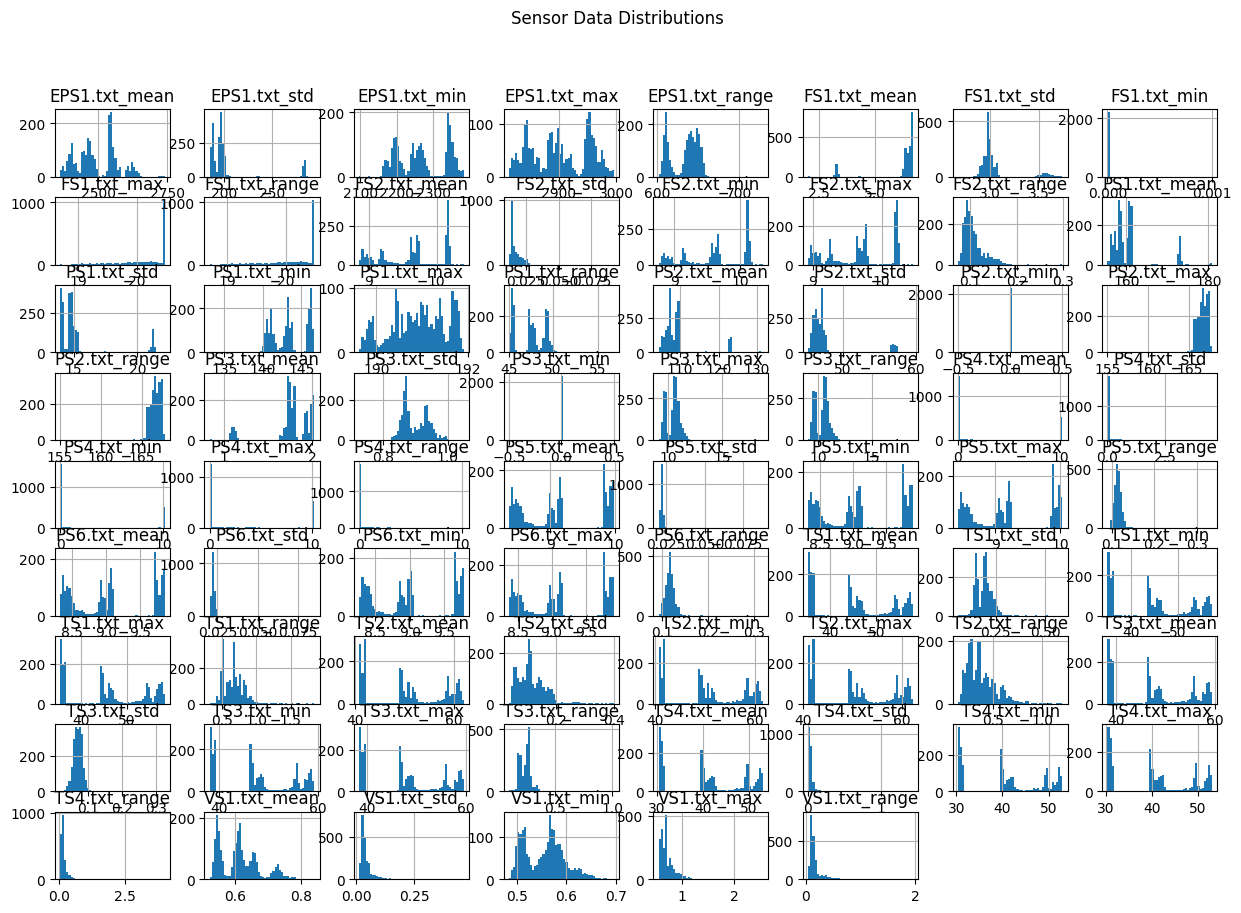
\includegraphics[width=0.4\textwidth]{sensor_data_distributions.png}  % Adjust width
        \caption{A plot showing the distribution of Extracted sensor data values across different categories.}
        \label{fig:example}
    \end{figure}
    \begin{figure}[htbp]  % 'htbp' controls the placement
        \centering
        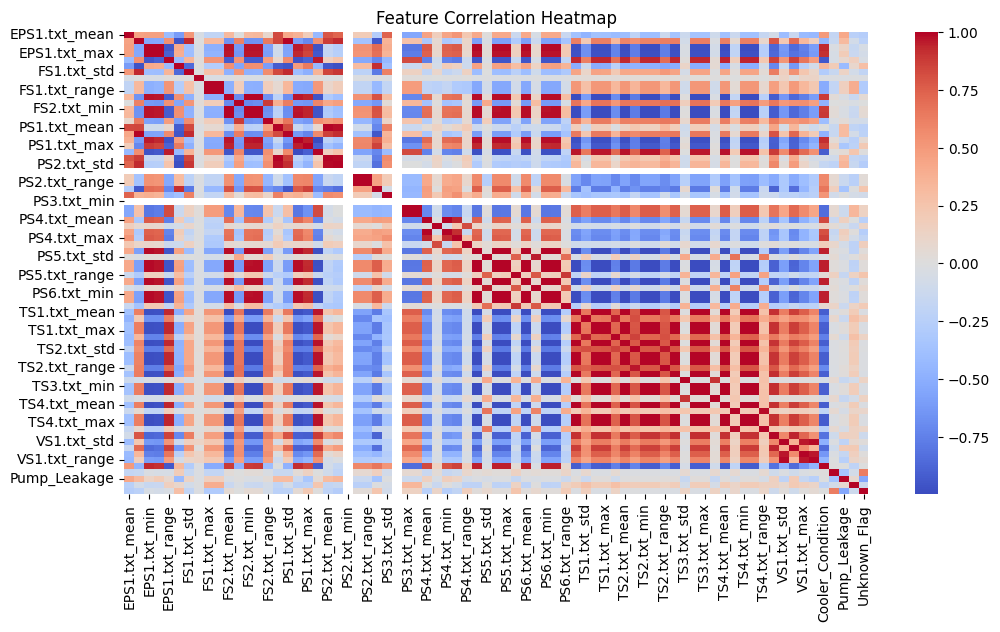
\includegraphics[width=0.4\textwidth]{feature_correlation_heatmap.png}  % Adjust width
        \caption{Feature correlation heatmap}
        \label{fig:example}
    \end{figure}
\end{itemize}

\subsection{Feature reduction using PCA} 
One of your goals is to improve efficiency for real-time prediction. Use Principal Component Analysis (PCA) to reduce the number of input features to speed up model training and model size.

\subsubsection{Code Snippet}
\begin{verbatim}
pca = PCA(n_components=10)
X_reduced = pca.fit_transform(X)
\end{verbatim}

\subsubsection{Output}
\begin{verbatim}
Original Feature Dimension: (2205, 70)
Reduced Feature Dimension: (2205, 10)
\end{verbatim}






\section{Model Training and Evaluation}
Two supervised machine learning models were trained to predict component failures based on sensor readings:

\subsection{Random Forest Classifier}
Random Forest, an ensemble learning method, was selected due to its interpretability and robustness against overfitting. The model was trained using 80\% of the dataset and evaluated on the remaining 20\%.

\textbf{Results:}
\begin{itemize}
    \item Accuracy: 99.77\%
    \item Precision, Recall, F1-score:
\end{itemize}
\begin{verbatim}
              precision    recall  f1-score   support

           0       1.00      1.00      1.00       228
           1       0.99      1.00      1.00       101
           2       1.00      0.99      1.00       112

    accuracy                           1.00       441
   macro avg       1.00      1.00      1.00       441
weighted avg       1.00      1.00      1.00       441
\end{verbatim}

\subsection{XGBoost Classifier}
XGBoost, a gradient boosting algorithm, was used to compare against the Random Forest model. XGBoost is known for handling complex relationships in data efficiently.

\textbf{Results:}
\begin{itemize}
    \item Accuracy: 99.09\%
    \item Precision, Recall, F1-score:
\end{itemize}
\begin{verbatim}
              precision    recall  f1-score   support

           0       0.99      1.00      1.00       228
           1       0.99      0.99      0.99       101
           2       0.99      0.97      0.98       112

    accuracy                           0.99       441
   macro avg       0.99      0.99      0.99       441
weighted avg       0.99      0.99      0.99       441
\end{verbatim}

\section{Evaluation}
\begin{itemize}
    \item \textbf{Classification Metrics}: Accuracy, Precision, Recall, F1-score.
    \item \textbf{Model Efficiency}: Training time and inference speed.
\end{itemize}

The results show that the Random Forest model performed slightly better in accuracy compared to XGBoost. Both models achieved near-perfect performance, indicating that the extracted features effectively captured the failure patterns in the dataset.

\section{Discussion}
\subsection{Project Timeline}
\begin{table}[h]
    \centering
    \begin{tabular}{|c|l|}
    \hline
    Week & Task \\
    \hline
    1 & Dataset exploration and preprocessing \\
    2-3 & Implement baseline models (Decision Trees, XGBoost) \\
    4 & Experiment with time-series models (LSTM, ARIMA) \\
    5 & Evaluation and performance comparison \\
    6 & Final report writing and refinements \\
    \hline
    \end{tabular}
    \caption{Project Timeline}
\end{table}

\subsection{Potential Challenges and Mitigations}
\begin{itemize}
    \item \textbf{Data Imbalance}: Rare failure cases may affect model performance.
    \begin{itemize}
        \item Solution: Apply oversampling techniques such as SMOTE.
    \end{itemize}
    \item \textbf{Computational Constraints}: Deep learning models may be resource-intensive.
    \begin{itemize}
        \item Solution: Prioritize lightweight models with feature selection.
    \end{itemize}
\end{itemize}

\section{Discussion and Future Work}
This study demonstrates that machine learning-based predictive maintenance can achieve near-perfect accuracy when applied to hydraulic system monitoring. Compared to previous research, our findings highlight the benefits of PCA in reducing computational overhead while maintaining predictive performance. Additionally, our comparative model analysis suggests that Random Forest offers a balance of interpretability and high accuracy, making it a strong candidate for real-time deployment.

\subsection{Future Directions}
Future work will focus on:
\begin{itemize}
    \item Extending this analysis to additional predictive models, such as deep learning-based architectures for time-series forecasting.
    \item Implementing real-time deployment strategies by optimizing model inference speed through quantization techniques.
    \item Exploring domain adaptation techniques to generalize the model to different hydraulic systems beyond the dataset used.
\end{itemize}

\section{Conclusion}
This project developed a predictive maintenance system for hydraulic systems using machine learning. By leveraging sensor data and feature engineering, the system successfully predicted failures with high accuracy while optimizing computational efficiency. Future work will aim to further refine deployment strategies for real-time industrial applications.


\end{document}

